%%%%     Please only edit bits which say to edit them     %%%%
%%%% They usually start with %///% to show where they are %%%%


%% Note: The font size for the template is set at 14 so it is nice and clearly readable. Please use small text sparingly.


%%% START : DO NOT EDIT %%%%

% Document setup
\documentclass[14pt]{extarticle}

\usepackage{graphicx,geometry,hyperref,enumitem,nicefrac,extsizes,color,nameref,calc,textcomp,csquotes,setspace}

\hypersetup{
    pdfborder={0 0 0}
}

% Important: This must come near the start of the setup file

\makeatletter
\newcommand*{\currentname}{\@currentlabelname}
\makeatother

\makeatletter
\def\normaljustify{%
  \let\\\@centercr\rightskip\z@skip \leftskip\z@skip%
  \parfillskip=0pt plus 1fil}
\makeatother

\setlength\parindent{0pt}
\setlength{\parskip}{\baselineskip}
\setcounter{secnumdepth}{2}
\setlength{\fboxsep}{0.4cm}
\setlength{\fboxrule}{0.04cm}

\definecolor{niceblue}{RGB}{166,218,255}
\definecolor{nicebluedark}{RGB}{0,104,179}
\definecolor{nicegreen}{RGB}{202,255,166}
\definecolor{nicegreendark}{RGB}{71,179,0}
\definecolor{nicered}{RGB}{255,166,166}
\definecolor{nicereddark}{RGB}{179,0,0}
\definecolor{niceyellow}{RGB}{255,254,166}
\definecolor{niceyellowdark}{RGB}{219,216,0}

\newcommand{\actioncol}{niceblue}
\newcommand{\notecol}{nicered}
\newcommand{\questioncol}{niceyellow}
\newcommand{\goalcol}{nicegreen}

\newcommand{\group}[1]{
    \begin{center}
    \parbox[c]{\linewidth} {
    	#1
    }
    \end{center}
}

\newcommand{\colourbox}[2]{
    \begin{center}
    \fcolorbox{#1dark}{#1}{
    	\parbox[c]{.9\linewidth} {
    	    #2 
    	}
    }
    \end{center}
}

\newcommand{\numberlist}[2][]{
    \begin{enumerate}[series=#1]
    	#2
    \end{enumerate}
    \vspace{-\topsep}
}

\newcommand{\resumenumberlist}[2]{
    \begin{enumerate}[resume=#1]
    	#2
    \end{enumerate}
    \vspace{-\topsep}
}

\newcommand{\itemlist}[1]{
    \begin{itemize}
    	#1
    \end{itemize}
    \vspace{-\topsep}
}

\newcommand{\valuelist}[2]{
    \begin{description}[align=left,labelwidth=*,leftmargin=#1]
    	#2
    \end{description}
}

\newcommand{\actions}[2][\currentname acs]{
    \colourbox{\actioncol}{ 
    	{\small\color{\actioncol dark} Actions}
    	\resumenumberlist{ #1 }{ #2 }
    }
}

\newcommand{\restartactions}[2][\currentname acs]{
    \colourbox{\actioncol}{ 
    	{\small\color{\actioncol dark} Actions}
    	\numberlist[#1]{ #2 } 
    }
}

\newcommand{\notes}[1]{
    \colourbox{\notecol}{ 
    	{\small\color{\notecol dark} Notes}\par
    	#1
    }
}

\newcommand{\questions}[2][questions]{
    \colourbox{\questioncol}{ 
    	{\small\color{\questioncol dark} Questions}
    	\resumenumberlist{ #1 }{ #2 } 
    }
}
\newcommand{\restartquestions}[2][questions]{
    \colourbox{\questioncol}{ 
    	{\small\color{\questioncol dark} Questions}
    	\numberlist[#1]{ #2 } 
    }
}
\newcommand{\goals}[1]{
    \colourbox{\goalcol}{ 
    	{\small\color{\goalcol dark} Goals}\par
    	#1 
    }
}

\newcommand{\boxesdescription}{
    \vspace{-\topsep}
    \begin{description}[align=left,labelwidth=*,leftmargin=3cm]
    	\item [{\color{\actioncol dark}Actions}] Stuff for you to do. They are highlighted in blue.
    	
    	\item [{\color{\notecol dark}Notes}] Notes about important stuff you need to be aware of (and possibly remember!). They are highlighted in red.
    	
    	\item [{\color{\questioncol dark} Questions}] Questions you should try to answer. Sometimes you'll need to write things down; other times you'll need to build something in the game. They are highlighted in yellow.

    	{\bfseries Ask a helper or the teacher to check your answers.}
    	
    	\item [{\color{\goalcol dark} Goals}] Stuff you should have completed at the end of each section. They are highlighted in green.
    \end{description}
}

\newcommand{\screenshot}[3][.9\linewidth-0.8cm]{
    \begin{center}
    \includegraphics[width=#1]{img/screenshots/#2}\par
    {\small #3}
    \end{center}
}

\newcommand{\image}[3][.9\linewidth-0.8cm]{
    \begin{center}
    \includegraphics[width=#1]{img/other/#2}\par
    {\small #3}
    \end{center}
}

\newcommand{\todo}[1]{
    \image[7cm]{todo}{#1}
}

\newcommand{\spacer}{
    \par\vspace{14pt}
}


%%% END : DO NOT EDIT %%%%

\usepackage[T1]{fontenc}%required
\usepackage{listings}
\lstset{ 
upquote=true,
columns=fullflexible,
literate={*}{{\char42}}1
         {-}{{\char45}}1
}
\usepackage{hyperref}

%///% Workshop info - edit these values for your workshop
\def\workshoptitle{What a Computer actually does}
\def\workshopsubtitle{The Big Hex Machine Assembly Worksheet}
\def\workshopauthor{Samuel Russell}

%%% START : DO NOT EDIT %%%%

\begin{document}

%% Note: The font type for the template is set to sans-serif (i.e. without the weird tick bits on the letters) so it is nice and clearly readable. Please use serif text (e.g. times new roman) sparingly.
%%          (The exception to this is for headers and one or two other places - mostly because I haven't figured out how to change them yet).
\sffamily

% Title page - do not edit
\begin{titlepage}

	\newgeometry{margin=2cm}
	
	\begin{figure}
	\centering
	\begin{minipage}{.5\textwidth}
		\centering
		
\includegraphics[width=.6\linewidth]{img/Bristol-University-Logo}
	\end{minipage}%
	\begin{minipage}{.5\textwidth}
		\centering
		
\includegraphics[width=.4\linewidth]{img/Digimakers}
	\end{minipage}
	
	\vspace{18pt}
	
	\end{figure}
	
	\centering
	\normalfont
	{\Large Merchant Venturers School of Engineering\par Outreach Programme\par}
	\vspace{2cm}
	\sffamily
	{\huge\bfseries\workshoptitle\par}
	\vspace{0.5cm}
	{\LARGE\bfseries\workshopsubtitle}
	
	\vfill
	
	{\normalsize Created by\par
	\large\slshape\workshopauthor}
	
	\vfill
	
	{\normalsize Organised by\par
	\large\href{mailto:Caroline.Higgins@bristol.ac.uk}{Caroline.Higgins@bristol.ac.uk}}

	\vfill

	{\large Published on \today\par}
\end{titlepage}

% Document setup - do not edit
\newgeometry{margin=1.5cm}

\renewcommand{\abstractname}{Notes to Teachers \& Helpers}
\begin{abstract}

\vspace{-\topsep}
    
\noindent
\vspace{-\topsep}
    
\setlist{leftmargin=0mm}
\itemlist {
    \setlength{\itemsep}{18pt}
    
%%% END : DO NOT EDIT %%%%
    
% Put notes to teachers and session helpers as a bullet point list in this section

%///% Begin editable content

    \item This workshop is intended to last 1\( \frac{1}{2} \) to 2 hours.
    
    \item This workshop is intended for ages 16\textsuperscript{+} (years 12\textsuperscript{+}).

    \item The content is intended to be learnt through using this worksheet as a guide.

    \item The learning platform is an on-line simulator hosted on Github.

    \item It can be used on any operating system with any modern internet browser.

    \item Students should already be comfortable with the idea of coding.\par This might be from a computing course at school or just self taught. They won't have used this language before but the worksheet tells them all they need to know.

    \item This workshop teaches the following skills:
    \valuelist{1cm}{
        \item [-] Logical thinking
    	\item [-] Appreciation of how computers really work
    }
    
% End editable content

%%% START : DO NOT EDIT %%%%

}

\end{abstract}

% Document setup - do not edit
\newgeometry{margin=1.5cm}


%%% END : DO NOT EDIT %%%%

% Sections from this point onwards are your choice, though Introduction, Conclusion (/Wrap-up/What we learnt) and Extra Resources sections are recommended.

%///% Begin editable content

\section*{Introduction to this worksheet}
This worksheet is split in to 3 sections. If you read \textbf{all} of them in turn everything should be clear. If not, try reading the previous sections and then ask a helper. 
\begin{itemize}
\item The first section tells you about the machine.
\item The second section contains exercises that introduce you to the different things you can do with the machine.
\item The third section challenges you use what you learnt in the exercises to write a program to solve some problems.
\end{itemize}

Note: Each exercise in the Exercises section is designed to be run on it's own. So when you try the next exercise you should either delete the old code or place a '\#' at the beginning of every line to \textit{comment it out}.

\section*{Introduction to the Big Hex Machine}
The Big Hex Machine is a two register machine with 32 kilobytes of RAM memory. However, it only supports 2 arithmetic operations: add and subtract. The other instructions move data to and from registers, RAM and IO ports. It is a bit big to have one each to play with but we have also build a on-line simulator so you can all try out writing programs for it!

\begin{center}
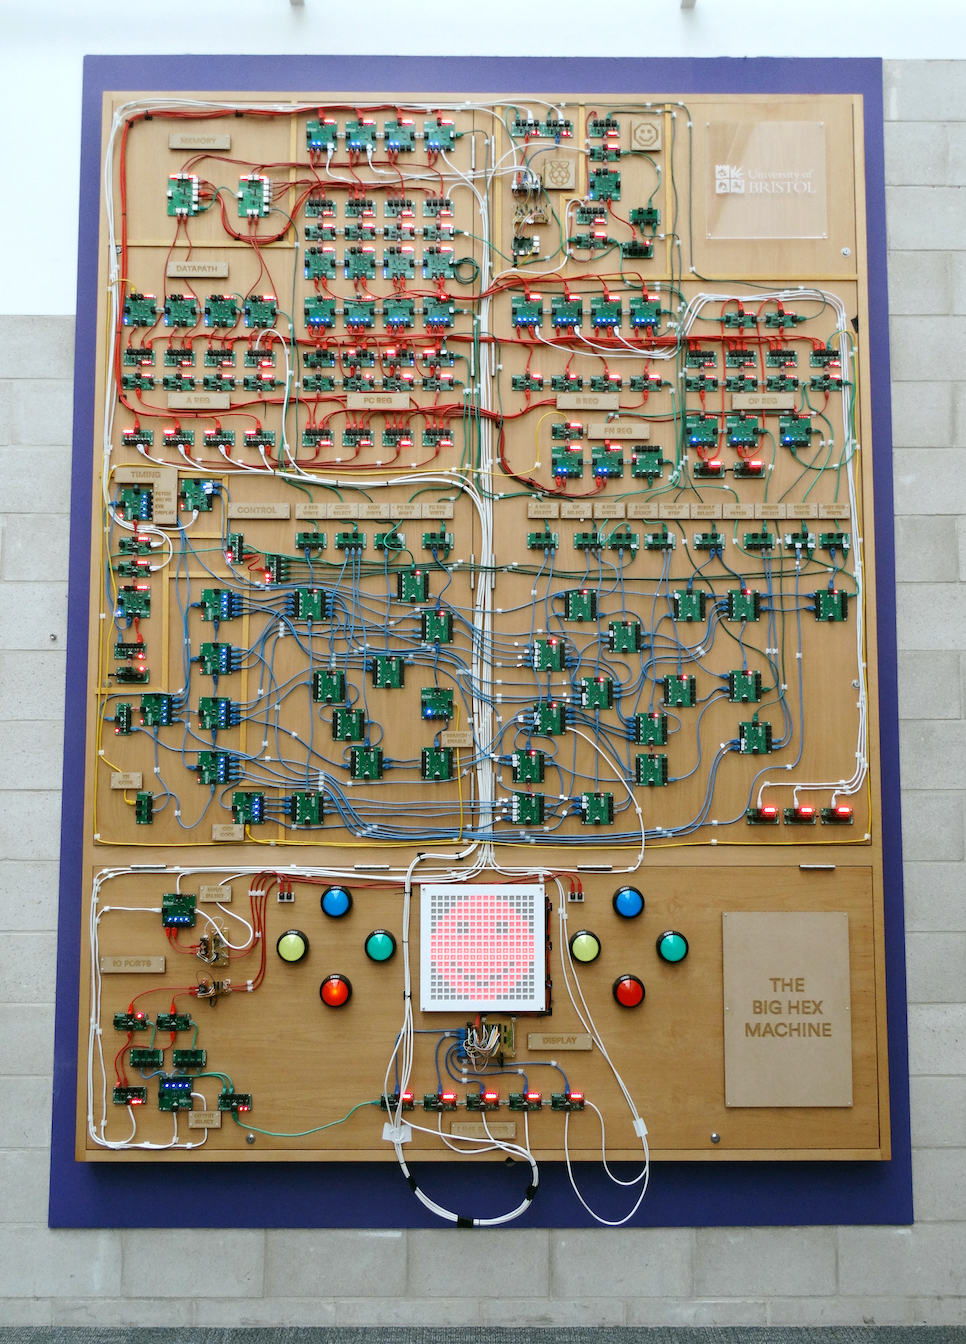
\includegraphics[width=10cm]{img/other/bighexmachine.jpg}\par
{\small The Big Hex Machine}
\end{center}

\section*{Introduction to the Instruction Set}
The the machine has 16 instructions, that each take one operand (a parameter), although they might also use the data stored in the registers. One of the instructions is split in to 4 different instructions (each without an operand) by giving one of 4 input operands. Don't worry, you won't need all of them and we'll take you through the ones you do, but if your interested \href{https://bighexmachine.github.io/BigHexOnlineSimulator/assemblySpec.pdf}{here} is the specification.\\

For the following exercises, X is a number either written in decimal like 182 (2 units, 8 tens, 1 hundred) or in hexadecimal like 0x298 (8 units, 9 sixteens, 2 sixteen-squareds).\\

We write an instruction with a it's short name (mnemonic) in capitals and then a space and then the operand/input value. For example to branch (move) one step forward in the program.
\begin{lstlisting}[frame=single]
BR 1
\end{lstlisting}

\break

\section*{Exercise 0}
Open up a web browser, and visit \href{http://tinyurl.com/bighexmachine}{tinyurl.com/bighexmachine}. A page will appear  that has 4 different sections:

\screenshot{main_page.png}{}

\begin{itemize}
\item A view of the memory. Each word (addressable slot) in memory is represented by  4 hexadecimal digits.
\item A view of the register values. The RA (register A) and RB (register B) are the important ones, but RP (program counter) also keeps track of where in the program you are.
\item A program control panel. This is where you can start and stop your program. It might be useful to step through one instruction at a time to see what is going on. But do remember to press reset each time you want to restart the program, other wise the computer will try and start up from where you left of last time.
\item A disassembler which translates the computer's binary in memory, back to human readable format. You will see every row says LDAM just because that happens to be the instruction represented by 00. 
\end{itemize}

\break

Click on 'edit', in the memory section.
On the left you can directly edit memory values, but we are going to use the area on the right to write our assembly programs.

\screenshot{edit_page.png}{}

When you have written some assembly code in the box you can click 'assemble' to translate the text in to machine code and then 'accept' to go back to the previous page to run and test your code. Read on to learn about how to write the assembly code!

\section*{Exercise 1: Inputting Values}
These are your basic instructions to put values in to the registers.
\begin{verbatim}
LDAC X	: Loads the value X in to register A
LDBC X	: Loads the value X in to register B
  (remember X is just a place holder for a number)
\end{verbatim}

Try writing something like the following, in the text box.
\begin{lstlisting}[frame=single]
LDAC 10
LDBC 0xA
\end{lstlisting}
Then click 'assemble' to translate the text in to machine code and then 'accept' to go back to main console. You can now run the program by clicking 'reset' then 'step' twice to execute each instruction in turn. Notice the instructions in the disassembler and the values change in the register viewer. Try changing the above code the load different values in to the registers.

\section*{Exercise 2: Adding Two Constants}

The OPR instruction is the instruction that is split in to 4 other instructions. One of these is ADD. 

\begin{verbatim}
OPR ADD : Adds the value in A reg to the value in B reg
          and puts the result in A reg.
OPR SUB : Subtracts the value in A reg by the value in 
          B reg and puts the result in A reg.
\end{verbatim}

\begin{lstlisting}[frame=single]
LDAC  1
LDBC  2
OPR    ADD
\end{lstlisting}

Again copy this in and have a play with different values and operations.

\section*{Exercise 3: Adding Two Values from Memory}

These are some instructions to get values from memory.

\begin{verbatim}
LDAM X : Gets the value at memory address X and puts it in register A
LDBM X : Gets the value at memory address X and puts it in register B
STAM X : Stores the value in register A in to memory at address X
\end{verbatim}

We can explicitly allocate addresses in memory by the DATA statement. Furthermore, these data portions can be named using a label and so the address X can be replaced the label word. Here is an example. Give it a go and see how it behaves. Note labels are written with a colon at the end.
\\
\begin{lstlisting}[frame=single]
LDAM  val_one
LDBM  val_two
OPR   ADD
STAM  val_out

val_one: DATA   0x10
val_two: DATA   2
val_out: DATA   0
\end{lstlisting}

\section*{Exercise 3: Loops and conditions}

This is where the real power of the computer comes; repeating stuff over and over, and making decisions!

This computer supports the unconditional branches (BR and BRB) which jumps in the program every time, and also conditional jumps (BRZ and BRN) which look at the value of the registers to decide to jump or not.
\begin{verbatim}
BR X  : Jumps X+1 places forward in the program.
        (remember it normally jumps 1 ahead anyway).
BRZ X : if A reg = 0 then it jumps as above but else jump goes
        to the next instruction like normal.
BRN X : if A reg < 0 then it jumps as above but else jump goes
        to the next instruction like normal.
BRB X : unconditionally jumps to position X.
\end{verbatim}

Just like we can label data we can also label parts of the program. This makes jumping to the right place easier.

Here's an example to try. Notice to never ending loop a the end.
\begin{lstlisting}[frame=single]
LDAC 10
start:
LDBC 1
OPR SUB
BRZ end
BR start
end:
BR end
\end{lstlisting}

\section*{Exercise 4: More Loops and conditions}
You may have to many variables to fit in to registers. If this is the case you have to store them in memory. This is called spilling and is normally done all automatically, but here is an example of it done in code.

\begin{lstlisting}[frame=single]
start:
LDAM counter
LDBC 1
OPR SUB
STAM counter
BRZ end
BR start
end:
BR end
counter:
DATA 10
\end{lstlisting}

\section*{Challenge 1: Summing}
Using the previous code examples, your challenge is to write a program to calculate the of sum the integers (whole numbers) from 1 to N. You can input the N using the LDAC/LDBC instructions.

\section*{Challenge 2: Multiplication}
This machine has a very \href{https://en.wikipedia.org/wiki/Reduced_instruction_set_computing}{RISC} architecture which means instructions can be decoded simply and the control
logic is relatively small. This does mean however that there is no multiplication instruction and so it has to be
done iteratively (in a loop, one step at a time). This was actually true in all most computers up until surprisingly recently.

Now can you create a program to multiple two numbers again setting the inputs with LDAC and/or LDBC.

Hint: This is quite similar to the previous code.

\section*{Challenge 2: Factorial}

This is a classic mathematical problem. Remember n! = (n) * (n - 1)...(2) * (1).

We can then use this multiplication code we have written as a sub procedure (function) to write a program that calculates the factorial of a
given number.

Hint: Use labels to name each part of the program, don't worry if it is in lots of sections. This actually makes a good program.

% Don't remove this... ;)
\end{document}
